\documentclass[border=4pt]{standalone}
\usepackage{amsmath,amssymb,xcolor,tikz}
\usetikzlibrary{arrows.meta,positioning,fit,backgrounds,calc}
\definecolor{frozengray}{HTML}{6B7280}\definecolor{trainedblue}{HTML}{2563EB}\definecolor{geogreen}{HTML}{059669}
\definecolor{froz}{HTML}{F3F4F6}\definecolor{trai}{HTML}{DBEAFE}\definecolor{geob}{HTML}{D1FAE5}
\newcommand{\metric}{AP$_{50}^{\text{axis+origin}}$}\newcommand{\apfifty}{AP$_{50}$}
\begin{document}
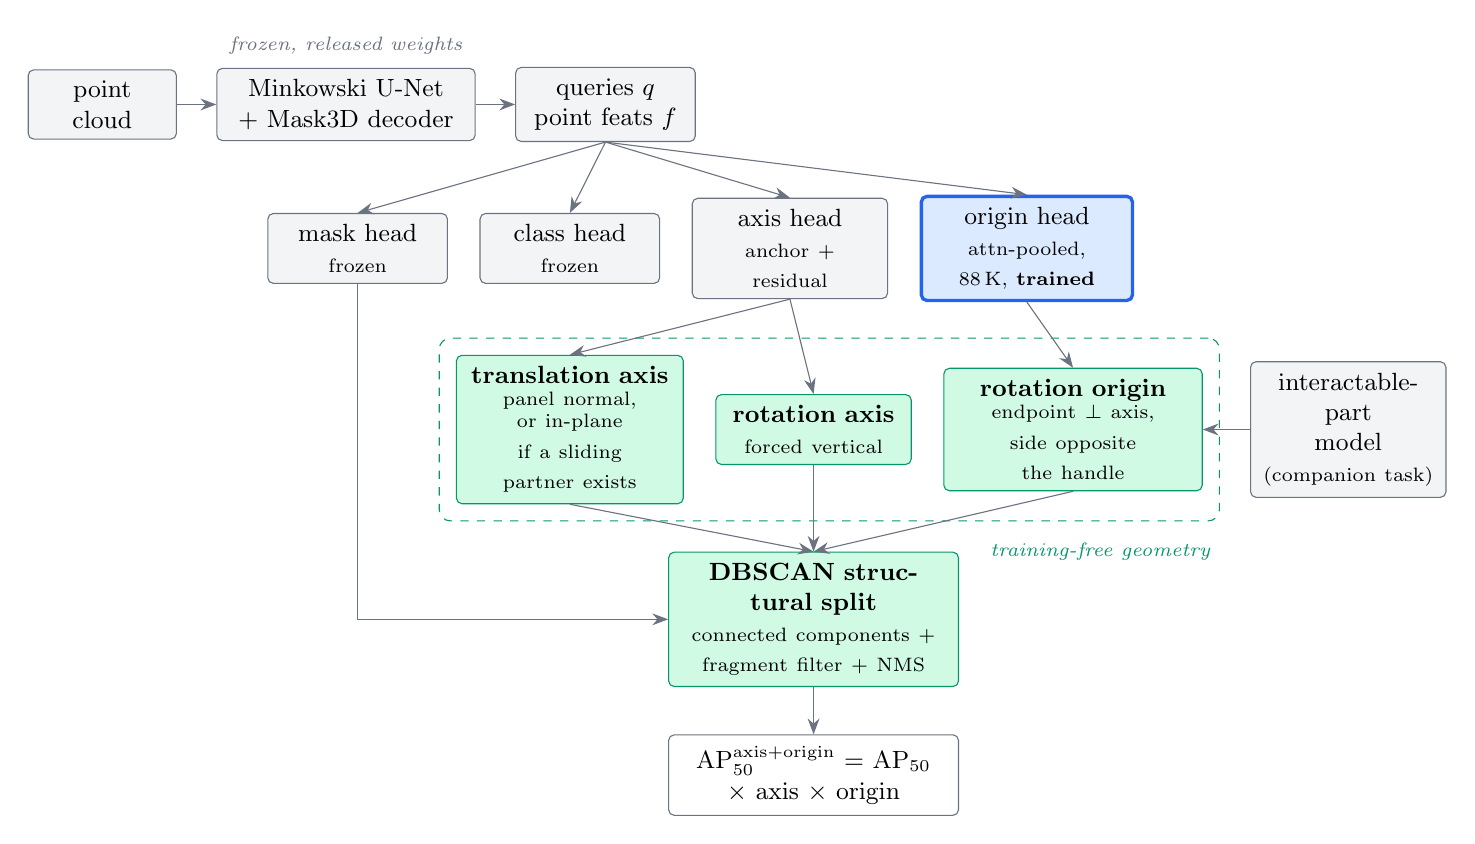
\begin{tikzpicture}[
  font=\small,
  box/.style={draw, rounded corners=2pt, align=center, inner sep=4pt,
              minimum height=8mm, text width=#1},
  froznode/.style={box=#1, fill=froz, draw=frozengray},
  trainode/.style={box=#1, fill=trai, draw=trainedblue, very thick},
  geonode/.style={box=#1, fill=geob, draw=geogreen},
  ar/.style={-{Stealth[length=2mm]}, draw=frozengray},
  lbl/.style={font=\scriptsize\itshape, text=frozengray},
]
\node[froznode=16mm] (pc) {point\\cloud};
\node[froznode=30mm, right=5mm of pc] (bb) {Minkowski U-Net\\ $+$ Mask3D decoder};
\node[froznode=20mm, right=5mm of bb] (feat) {queries $q$\\ point feats $f$};
\draw[ar] (pc) -- (bb); \draw[ar] (bb) -- (feat);
\node[lbl, above=0.5mm of bb] {frozen, released weights};
\node[froznode=20mm, below left=9mm and 20mm of feat.south] (mh) {mask head\\\scriptsize frozen};
\node[froznode=20mm, right=4mm of mh] (ch) {class head\\\scriptsize frozen};
\node[froznode=22mm, right=4mm of ch] (ah) {axis head\\\scriptsize anchor $+$ residual};
\node[trainode=24mm, right=4mm of ah] (oh) {origin head\\\scriptsize attn-pooled, 88\,K, \textbf{trained}};
\foreach \n in {mh,ch,ah,oh} \draw[ar] (feat.south) -- (\n.north);
\node[geonode=26mm, below=9mm of ch] (gtr) {\textbf{translation axis}\\\scriptsize panel normal, or in-plane\\\scriptsize if a sliding partner exists};
\node[geonode=22mm, right=4mm of gtr] (grot) {\textbf{rotation axis}\\\scriptsize forced vertical};
\node[geonode=30mm, right=4mm of grot] (gor) {\textbf{rotation origin}\\\scriptsize endpoint $\perp$ axis,\\\scriptsize side opposite the handle};
\draw[ar] (ah.south) -- (gtr.north); \draw[ar] (ah.south) -- (grot.north); \draw[ar] (oh.south) -- (gor.north);
\node[froznode=22mm, right=6mm of gor] (hnd) {interactable-part\\model\\\scriptsize (companion task)};
\draw[ar] (hnd.west) -- (gor.east);
\begin{scope}[on background layer]
  \node[fit=(gtr)(grot)(gor), draw=geogreen, dashed, rounded corners, inner sep=6pt] (geobox) {};
\end{scope}
\node[lbl, text=geogreen, anchor=north east] at ([yshift=-1.5mm]geobox.south east) {training-free geometry};
\node[geonode=34mm, below=11mm of grot] (dbs) {\textbf{DBSCAN structural split}\\\scriptsize connected components $+$ fragment filter $+$ NMS};
\draw[ar] (gtr.south) -- (dbs.north); \draw[ar] (grot.south) -- (dbs.north); \draw[ar] (gor.south) -- (dbs.north);
\draw[ar] (mh.south) |- (dbs.west);
\node[box=34mm, below=6mm of dbs, draw=frozengray, fill=white] (out) {\metric{} $=$ \apfifty{} $\times$ axis $\times$ origin};
\draw[ar] (dbs) -- (out);
\end{tikzpicture}
\end{document}
